\section{REFERENCIAL TEÓRICO}
\label{cap:referencial_teorico}

Neste capítulo é apresentado o referencial teórico para desenvolvimento deste trabalho. Descreve-se a triangulação de Delaunay e o seu dual, o diagrama de Voronoi, na seção (\ref{cap_triangulacao_delaunay}). Também apresenta-se, nessa seção, algoritmos para geração, manutenção e refinamento de malhas de Delaunay.

Na seção (\ref{cap_discretizacao_equacao_calor}), realiza-se a discretização da equação do calor, utilizando-se o método dos volumes finitos com o diagrama de Voronoi e define-se um algoritmo em forma de pseudocódigo referente a essa discretização. 

Na seção (\ref{cap_metodo_gradientes_conjugados}), tem-se a construção do método dos gradientes conjugados, apresentando-se um pseudocódigo. Com o intuito de se diminuir o número de iterações, também expõe-se nessa seção uma forma de pré-condicionamento da matriz de coeficientes e um algoritmo para reordenação dos vértices, o algoritmo de Cuthill-McKee reverso em conjunto com o algoritmo de vértice pseudoperiférico.

Na seção (\ref{cap_suavizacao_laplaciana}), descreve-se a suavização laplaciana. Também são apresentadas técnicas de melhoria da qualidade da malha utilizando a suavização laplaciana.

Na seção (\ref{cap_malhas_moveis}), aborda-se as principais características sobre malhas móveis, como adaptatividade de malhas, o princípio de equidistribuição, também apresentando diferentes trabalhos que pretendem solucionar equações diferenciais parciais por diferentes métodos, utilizando os mais variados tipos de malhas. Também apresentam-se técnicas de movimento dos vértices baseadas na formulação laplaciana.

Na seção (\ref{cap_metrica_geometrica}), explana-se uma métrica geométrica para verificar a degeneração da malha ao movimentar os vértices.

\subsection{A triangulação de Delaunay e o diagrama de Voronoi}
\label{cap_triangulacao_delaunay}

Nesta seção, aborda-se a triangulação de Delaunay e o diagrama de Voronoi. Também são apresentados algoritmos de construção, manutenção e refinamento dessa triangulação.

\subsubsection{Considerações iniciais}

Uma malha pode ser classificada de acordo com a disposição relativa dos diferentes elementos existentes. Uma malha {\it estruturada} é caracterizada pela sua conectividade {\it regular}. Isso significa que, a posição dos nós pode ser mapeada de modo a definir quais nós serão vizinhos por meio de cálculo. Isso pode restringir as escolhas dos elementos para quadriláteros em 2D ou hexaedros em 3D. Se os nós não podem ser arranjados de tal forma, a malha é dita {\it não estruturada} ou {\it irregular}. Em uma malha irregular, deve-se armazenar a conexão entre os nós que formam a malha. Os elementos podem ser, em sua forma básica, triângulos ou tetraedros em 2D e 3D, respectivamente, bem como hexaedros, ou qualquer outra forma, em malhas mais complexas. \cite[p.~20]{Thompson1999}.

Na busca de se atingir uma determinada qualidade na aproximação, com desempenho computacional aceitável, ao longo das últimas décadas, pesquisas têm sido realizadas em técnicas de geração e refinamento de malhas, como por exemplo em \citeonline{Preparata1985, Thompson1999, Teng2000, Chen2004, George2008}. Ainda em problemas com domínios com geometria complexa, a geração da malha pode ser uma tarefa dispendiosa. Uma forma de se obter uma malha de qualidade a baixo custo computacional é a utilização da triangulação Delaunay. 

A triangulação de \citeonline{Delaunay1939} é um tipo de malha irregular. Com uma triangulação de Delaunay, maximiza-se o menor ângulo da triangulação. Obtém-se triângulos com ângulos não próximos a $0^{\circ}$ e a $180^{\circ}$. Em esquemas numéricos, triângulos com ângulos próximos a $0^{\circ}$ e $180^{\circ}$ são considerados de má qualidade, levando a resultados imprecisos. 

A triangulação de Delaunay possui a característica de unicidade, de forma que, dado um conjunto de vértices, a triangulação é sempre única, exceto em casos degenerados, nos quais quatro ou mais vértices são cocirculares, existindo duas possibilidades de triangulação (local). Cada uma das duas possibilidades de triangulação que divide o quadrilátero em dois triângulos satisfaz a ``condição Delaunay'', isto é, em que o circuncírculo (único círculo que passa pelos vértices do triângulo) é vazio. Essa noção pode ser estendida a três dimensões.

Um diagrama de \citeonline{Voronoi1908} é uma decomposição (em partições) de um espaço em torno de um vértice. Cada polígono consiste em uma região de espaço que fica mais próxima de cada vértice do que qualquer outro vértice gerador do diagrama de Voronoi, que é formado pelos polígonos de Voronoi. Diversos algoritmos para a geração do diagrama de Voronoi foram desenvolvidos. São exemplos desses algoritmos, \citeonline{Shamos1975}, que desenvolveram um algoritmo O($n\cdot \mbox{lg}(n)$) por divisão-e-conquista e \citeonline{Green1978}, que produziram um algoritmo O($n^2$) por inserção incremental, em que $n$ é a quantidade de vértices da triangulação.

Uma partição do diagrama de Voronoi e a triângulação de Delaunay correspondente pode ser observada na figura (\ref{fig_malha_voronoi}).

\begin{figure}[!ht]
  \centering
  \includegraphics[width=150pt]{imagens_discretizacao/malha_voronoi.png}
  \caption{\footnotesize{Em azul, arestas de uma partição do diagrama de Voronoi e, em vermelho, os triângulos de Delaunay correspondentes.
}}
  \label{fig_malha_voronoi}
\end{figure}

\subsubsection{Manutenção da triangulação de Delaunay - Algoritmo de Lawson}
\label{cap_algoritmo_lawson}
Para construção da triangulação Delaunay, pode-se utilizar o algoritmo de \citeonline{Lawson1977}, um algoritmo de complexidade $O(n^2)$. Esse algoritmo é utilizado para gerar ou para manter uma triangulação de Delaunay. Sua escolha deve-se à sua facilidade de implementação.

A partir de uma triangulação inicial, verifica-se se todas as arestas que compõem a triangulação atendem aos critérios da triangulação de Delaunay. Caso essas arestas não atendam aos critérios da triangulação de Delaunay, realiza-se o {\it flip}. 

O {\it flip} é um procedimento, definido por \citeonline{Lawson1977}, em que ocorre a inversão da aresta invadida, conforme demonstrado na figura (\ref{fig_flip}). Com o {\it flip}, uma nova aresta é criada e, em seguida, verifica-se, recursivamente, essa aresta e os dois triângulos que a compartilham. O algoritmo termina quando todas as arestas atendem aos critérios da triangulação de Delaunay, ou seja, são localmente de Delaunay.  

\begin{figure}[!ht]
  \centering
  \includegraphics[width=350pt]{imagens_delaunay/novo_flip.png}
  \caption{\footnotesize{Aplicação do algoritmo de Lawson: (a) Uma aresta invadida, mostrada em vermelho, que não é de Delaunay, é verificada. (b) O algoritmo do {\it flip} é aplicado para inverter a aresta invadida, tornando-a localmente de Delaunay. (c) Verifica-se se essa aresta e os dois triangulos que a compartilham são localmente de Delaunay. Como a aresta não é invadida, essa é mostrada em azul.
}}
  \label{fig_flip}
\end{figure}

No algoritmo (\ref{algoritmo_lawson}) tem-se um pseudocódigo referente ao algoritmo de \citeonline{Lawson1977}.

\begin{algorithm}[!ht]
\caption{Algoritmo de Lawson.} 
\label{algoritmo_lawson}
\Entrada{Triangulação $T$.}
\Saida{Triangulação de Delaunay $T$.}
  \Inicio{
    \Para {(cada aresta $\overline{ab} \in T$)} {
    \CommentSty{// Efetua teste do circuncírculo.} \\
      \Se {($\overline{ab}$ não é localmente de Delaunay)} {
	  Sejam $\Delta abc$ e $\Delta abd$ os triângulos que compartilham $\overline{ab}$; \\
	  Trocar $\overline{ab}$ por $\overline{cd}$; \CommentSty{// Realiza o {\it flip} da aresta.}\\
      }
    }
    \Retorna {$T$;}
  }
\end{algorithm} 

\subsubsection{Construção da triangulação de Delaunay - Algoritmo de Green-Sibson}
\label{cap_algoritmo_green_sibson}

O algoritmo de Green-Sibson foi proposto por \citeonline{Green1978} para gerar o diagrama de Voronoi, porém, pode ser facilmente adaptado para gerar a triangulação de Delaunay. A partir de uma triangulação de Delaunay inicial realiza-se a inserção incremental de vértices.  Os pontos inseridos na triangulação de Delaunay são chamados de pontos de {\it  Steiner}. A complexidade desse algoritmo é $O(n^2)$.

Nesse algoritmo, ocorre a inserção de um vértice por vez e, a cada inserção, verifica-se se o novo vértice encontra-se sobre uma aresta ou dentro de um triângulo. Caso o novo vértice $e$ se localize dentro do triângulo $\Delta abc$, liga-se $e$ aos três vértices do triângulo que o contém, criando-se três novos triângulos, $\Delta abe$, $\Delta ace$ e $\Delta bce$. Caso o novo vértice $f$ se localize sobre uma aresta $\overline{de}$, deve-se dividir $\overline{de}$ em duas novas arestas. Considere $\Delta bde$ e $\Delta cde$ os triângulos que compartilham $\overline{de}$. Divide-se a aresta $\overline{de}$ em duas novas arestas, $\overline{ef}$ e $\overline{df}$. Em seguinda, liga-se $f$ aos vértices $b$ e $c$, opostos à aresta $\overline{de}$, pertencentes aos triângulos que compartilham $\overline{de}$, criando-se quatro novos triângulos, $\Delta bef$, $\Delta bdf$, $\Delta cef$ e $\Delta cdf$. Em ambos os casos realiza-se o teste do circuncírculo após a geração das novas arestas, utilizando o algoritmo de \citeonline{Lawson1977} para manutenção da malha. Se existirem arestas invadidas, realiza-se o {\it flip}. O algoritmo termina quando não existirem arestas invadidas. Na figura (\ref{fig_green_sibson}), pode-se observar um exemplo de execução do algoritmo de \citeonline{Green1978} 

No algoritmo (\ref{algoritmo_green_sibson}) tem-se um pseudocódigo referente ao algoritmo de \citeonline{Green1978}.

\begin{figure}[!ht]
  \centering
  \includegraphics[width=350pt]{imagens_delaunay/green_sibson.png}
  \caption{\footnotesize{Aplicação do algoritmo de Green Sibson: (a) Tem-se a malha inicial com a inserção de um novo vértice que localiza-se dentro de um triângulo. (b) Divide-se o triângulo gerando três novos triângulos, formados pelas arestas em azul. (c) Realiza-se o teste dos circuncírculos e encontra-se uma aresta invadida, mostrada em vermelho. (d) Efetua-se o {\it flip} na aresta invadida. (e) Realiza-se o teste dos circuncírculos. (f) Ocorre a inserção de um novo vértice localizado sobre uma aresta. (g) Ocorre a divisão da aresta que contém o novo vértice, gerando quatro novos triângulos, compostos pelas novas arestas em azul. (h) Realiza-se o teste dos circuncírculos e verifica que não existe aresta invadida.
}}
  \label{fig_green_sibson}
\end{figure}

\begin{algorithm}[!ht]
\caption{Algoritmo de Green-Sibson.} 
\label{algoritmo_green_sibson}
\Entrada{Triangulação de Delaunay $TD$ e lista $L_V$ de vértices a serem inseridos em $TD$.}
\Saida{$TD$ com os vértices pertencentes à $L_V$.}
  \Inicio{
    \Para {(todo vértice $v \in L_V$)} {
	Inserir $v$ em $TD$; \\
	\eSe {($v$ localiza-se sobre aresta $\overline{ab} \in TD$)} {
	    Sejam $\Delta abc$ e $\Delta abd$ os triângulos que compartilham $\overline{ab}$; \\
	    Criar as arestas $\overline{av}$, $\overline{bv}$, $\overline{cv}$, $\overline{dv}$ e inserir em $TD$; \\
	}
	{
	    Seja $\Delta abc$ o triângulo que contém $v$; \\
	    Criar as arestas $\overline{av}$, $\overline{bv}$, $\overline{cv}$ e inserir em $TD$; \\
	}
    }
    \Para {(cada aresta $\overline{ab}$ criada)} {
	AlgoritmoLawson($\overline{ab}$);\\
    }
    \Retorna {$TD$;}
  }
\end{algorithm} 

\subsubsection {Refinamento de Delaunay} 
\label{cap_algoritmos_refinamento}
Nesta seção, são apresentados dois algoritmos no estado da arte para o refinamento de Delaunay: algoritmo de \citeonline{Ruppert1995} e \emph{off-centers} \cite{Ungor2004, Ungor2009, Oliveira2012a}.


\textbf {Algoritmo de Ruppert}
\label{cap_algoritmo_ruppert}

O algoritmo de \citeonline{Ruppert1995} garante que todos os triângulos pertencentes à triangulação terão ângulos entre $\alpha$ e $\pi-2\alpha$, de forma que $\alpha$ pode ser um ângulo máximo de aproximadamente 20,7 graus. Ao se inserir um vértice na triangulação, duas operações são possíveis: dividir um segmento e dividir um triângulo. Ao se dividir um segmento, um vértice é inserido em seu ponto médio. Ao se dividir um triângulo, um vértice é inserido em seu circuncentro. Com isso, uma nova triangulação é realizada \cite{Oliveira2012a}. 

Um algoritmo para a geração da triangulação de Delaunay pode utilizar uma medida de qualidade. Uma possível medida de qualidade chama-se \emph{Circunradius-to-shortest Edge Radio} (CER), que é definida pela razão do raio do circuncírculo \emph{r} (\emph{circunraio}) do triangulo, pela menor aresta \emph{l} do triângulo. É especificado um limite superior $\rho=r/l$ para o CER de todos os triângulos da malha. A razão $\rho$ de um triângulo está relacionada com seu menor ângulo ${\alpha}$ pela fórmula ${\rho = 1/[2\cdot sen(\alpha)]}$. Quanto menor for a razão $\rho$, maior será o ângulo $\alpha$ do triângulo. Esse limite superior $\rho$ garantirá que não há triângulo na malha com ângulo menor que ${\arcsin(1/2\rho)}$ \cite{Pebay2003}. 

Esse algoritmo pode receber como parâmetro de entrada um grafo planar de linhas não curvas (\emph {Planar Straight Line Graph} - PSLG). Um PSLG é um conjunto de vértices e seus segmentos. Segmentos são arestas que não podem ser removidos. Claramente, os segmentos não se interceptam. Um segmento é considerado invadido quando um vértice incide dentro de seu círculo diametral. Um pseudocódigo referente ao algoritmo de \citeonline{Ruppert1995} é apresentado no algoritmo (\ref{algoritmo_ruppert}).

\begin{algorithm}[!ht]
\caption{Refinamento de Ruppert.} 
\label{algoritmo_ruppert}
\Entrada{PSLG $G$.}
\Saida{Triangulação de Delaunay de $G$ com todos os $\measuredangle \geq \alpha$.}
\Inicio{
    Adicionar um delimitador quadrado $D$ à $G$: \\
    \Inicio{
      Calcular os extremos de $G$: $x_{min}$, $y_{min}$, $x_{max}$, $y_{max}$; \\
      Seja $span(G) = \max(x_{max} - x_{min}, y_{max} - y_{min})$; \\
      Seja $D$ o quadrado de lado $3 \times span(G)$, centralizado em $G$;\\
      Adicionar os quatro segmentos de contorno de $D$ à $G$; \\
    }
    Seja a lista de segmentos $L_{S} =$ arestas de $G$; \\
    Seja a lista de vértices $L_{V} =$ vértices de $G$; \\
    Construir a triangulação de Delaunay inicial $TD(L_{V})$;\\
    \Repita{ (at\'e que nenhum segmento esteja invadido e nenhum $\measuredangle < \alpha$) } 
    {
        \CommentSty{// Divide todos os segmentos invadidos em seu\\ // ponto m\'edio.}  \\  
	\Enqto{ (existe algum segmento $s \in L_{S}$ invadido) }
	{
	    $DividirSegmento(s)$; 
	}
	\CommentSty{ // Verifica tri\^angulos com $\measuredangle  < \alpha$.}  \\  
	\Enqto{ (existe algum tri\^angulo $\delta \in TD(L_{V})$ com $\measuredangle  < \alpha$;) }
	{
	    Seja $c$ o circuncentro de $\delta$; \\   	    
	    \eSe { ($c$ invade algum segmento $s \in L_{S}$) } 
	    {		
	        \CommentSty{// Divide todos os segmentos invadidos\\ // em seu ponto m\'edio.}  \\  
		$DividirSegmento(s)$; \\
	    }	    
	    {
	        \CommentSty{// Divide tri\^angulos com $\measuredangle < \alpha$, em seu\\ // circuncentro, adicionando $c$ \`a $L_{V}$.}  \\  
		$DividirTriangulo(\delta)$; \\
	    }   
	}
    }
    \Retorna {Triangulação de Delaunay corrente $TD(L_{V})$;}
}
\end{algorithm}  

Nas situações em que o PSLG possui ângulos menores que $90^{\circ}$, o algoritmo tende a formar triângulos com ângulos muito agudos. \citeonline{Shewchuk1997} provou que o algoritmo irá parar para qualquer entrada com ângulos de, no mínimo, $60^{\circ}$.

\textbf {\emph{Off-centers}}
\label{cap_off_centers}

\citeonline{Ungor2004,Ungor2009} propôs um refinamento de Delaunay similar ao algoritmo de \citeonline{Ruppert1995}. Em seu trabalho, introduz-se um novo tipo de pontos de {\it Steiner}, chamados {\it off-centers}, como uma alternativa aos circuncentros, apresentando um novo algoritmo de refinamento de Delaunay. Caso um triângulo seja considerado de má qualidade, pela medida CER, o algoritmo tenta inserir o \emph{off-center}. Caso o \emph{off-center} invada algum segmento, então, o novo vértice é inserido no ponto médio desse segmento em vez do \emph{off-center}. Um pseudocódigo referente a esse algoritmo pode ser observado no algoritmo (\ref{algoritmo_ungor}).

\begin{algorithm}[!ht]
\caption{Refinamento de \"Ungor.} 
\label{algoritmo_ungor}
\Entrada{PSLG $G$.}
\Saida{Triangulação de Delaunay de $G$ com todos os $\measuredangle \geq \alpha$.}
\Inicio{
    Seja $TD$ a triangulação de Delaunay dos vértices de $G$; \\
    Calcular: \\
    \ \ $B = $candidados à {\it off-centers} que invadem algum segmento;\\
    \ \ $C = $candidados à {\it off-centers} que não invadem segmentos;\\
    \ \ $D = $candidados à ponto médio;\\
    \Enqto{ ($C \cup D) \neq$ vazio }
    {
	Escolher um ponto $c_{o} \in (C \cup D)$ e inserir $c_{o}$ na triangulação $TD$; \\ 
	\Se { ($c_{o}$ é ponto médio de um segmento $s$)}
	{
	    $DividirSegmento(s)$;\\
	}
	Atualizar $TD$ e recalcular $B$, $C$ e $D$;
    }    
    \Retorna {Triangulação de Delaunay corrente $TD$;}    
}
\end{algorithm}  

Para calcular o {\it off-center}, considera-se um triângulo $\delta$, de má qualidade, formado pelos vértices $p$, $q$ e $r$. A menor aresta de $\delta$ é $pq$ e o seu circuncentro é $c$. O {\it off-center} $c_{o}$ de $\delta$ é o seu circuncentro se o CER do triângulo formado pelos vértices  $p$, $q$ e $c$ for menor ou igual a um dado limite $\rho_{\alpha}$, em que $\rho_{\alpha}$ é a medida CER de um ângulo $\alpha$, conforme mostrado na figura (\ref{fig_off_center}.a). Caso contrário, o {\it off-center} $c_{o}$ será o ponto na bissetora da aresta, dentro do circuncírculo, que faz com que o CER do triângulo $\Delta pqc_{o}$ seja exatamente igual a $\rho_{\alpha}$. A bissetora da aresta é a linha que passa pelo ponto médio de uma aresta de um triângulo e pelo seu circuncentro. 

O círculo que passa pelos vértices da menor aresta $pq$, centrado no {\it off-center}, é chamando {\it off-circle}. Caso o triângulo $\delta$ tivesse duas arestas menores iguais, escolheria-se uma delas, arbitrariamente. 

\begin{figure}[!ht]
  \centering
  \includegraphics[width=300pt]{imagens_delaunay/off-center_A_B_rotulado.png}
  \caption{\footnotesize{ O {\it off-center} e o circuncentro do triângulo $\delta$, formado pelos vértices $p$, $q$ e $r$, são, respectivamente, $c_{0}$ e $c_{1}$. O circuncentro do triângulo formado pelos vértices $p$, $q$ e $c_{0}$ é $c_2$. Se $|c_{0} c_{2}| \leq \rho_{\alpha}|pq|$ então $c_{0} = c_{1}$, que é demonstrado em (a). Caso contrário, $c_{0} \neq c_{1}$. Nesse caso, calcula-se $c_{2}$ de forma que $|c_{0} c_{2}| = \rho_{\alpha}|pq|$, que é demonstrado em (b). O {\it off-circle} do triângulo $\delta$ é o circuncírculo em (a) e é mostrado em linhas tracejadas em (b). Figura adaptada de \citeonline{Ungor2004, Ungor2009}.
}}
  \label{fig_off_center}
\end{figure}

\citeonline{Ungor2004,Ungor2009} mostrou que seu algoritmo possui as mesmas garantias do algoritmo de Ruppert. Seus experimentos mostraram que seu algoritmo insere aproximadamente 40\% menos vértices que outros algoritmos de inserção no circuncentro e malhas 30\% menores em relação ao número de elementos.

\subsubsection{Resumo}

Nesta seção, apresentou-se a triangulação de Delaunay, um tipo de malha irregular que possui a propriedade de maximizar o menor ângulo da triangulação e o seu dual, o diagrama de Voronoi. 

Nas subseções (\ref{cap_algoritmo_lawson}), (\ref{cap_algoritmo_green_sibson}) e (\ref{cap_algoritmos_refinamento}) foram explanados um algoritmo para manutenção da triangulação de Delaunay, o algoritmo de \citeonline{Lawson1977}, um algoritmo para construção da triangulação de Delaunay, o algoritmo de \citeonline{Green1978}, e dois algoritmos para refinamento de Delaunay: o algoritmo de \citeonline{Ruppert1995} e \citeonline{Ungor2004,Ungor2009}.

\subsection{Discretização da equação do calor}
\label{cap_discretizacao_equacao_calor}

Nesta seção, aborda-se a discretização da equação do calor utilizando-se o método dos volumes finitos com o diagrama de Voronoi. Também mostra-se um pseudocódigo referente a esse método.

\subsubsection{Considerações iniciais}

No método dos volumes finitos (MVF), o domínio do problema é dividido em um conjunto finito de volumes, adjacentes entre si, chamados de volumes de controle (VC). Nesse método, realiza-se um balanço de conservação da propriedade em questão, para cada volume elementar, de modo a se obter a equação aproximada, respeitando-se a lei de conservação. Há interesse na aplicação do método dos volumes finitos na solução de equações diferenciais parciais (EDPs) devido a essa característica.

Uma forma de se obter as equações aproximadas no MVF é integrar, sobre cada volume elementar, no espaço e no tempo, as equações na forma conservativa, ou divergente. Nessa forma, os termos relacionados aos fluxos aparecem dentro das derivadas em relação às coordenadas espaciais. Ao realizar a integração para todos os VCs, obtém-se uma equação algébrica para cada volume e, consequentemente, obtém-se um sistema de equações algébricas. Esse sistema de equações é formado pelas variáveis localizadas nos centróides dos VCs. Para as aproximações, utilizam-se funções de interpolação por meio dos valores das variáveis dos VCs vizinhos. Devido a sua generalidade, qualquer tipo de malha pode ser utilizada, regular ou irregular \cite[p. 27 - 33]{Maliska2010}.

Na seção (\ref{cap_equacao_calor}), apresenta-se o modelo matemático para difusão de fluidos. Na seção (\ref{cap_discretizacao_malha_irregular}), é tratada a discretização da equação do calor com o diagrama de Voronoi e apresenta-se o pseudocódigo dessa discretização.

\subsubsection{Equação do calor}\label{cap_equacao_calor}

A equação do calor é um modelo matemático para a difusão de calor em sólidos, ou seja, descreve o fluxo de calor em um corpo sólido. Esse modelo consiste em uma equação de derivadas parciais que, muitas vezes, é também chamada de equação de difusão. Essa equação, em sua forma generalizada, é definida como

\begin{equation}
\frac {\partial } {\partial t} (\rho \phi)  =  \nabla \cdot \left( \frac {k} {c_{p}} \nabla \phi \right) ,
\label{equacao_diferencial_calor_forma_geral}
\end{equation}

\noindent em que $\phi$ é a temperatura, $t$ é o tempo, $\rho$ é a massa volumétrica do material, $c_{p}$ é o seu calor específico e $k$ é a condutibilidade térmica. 

Segundo \citeonline[p. 73]{Tannehill1997}, pode-se integrar a equação (\ref{equacao_diferencial_calor_forma_geral}) sobre um volume $V$ qualquer obtendo-se

\[
\iiint_V  \left ( \frac {\partial } {\partial t} (\rho \phi)  +  \nabla \cdot {\mathbf q} \right )dV = 0,
\]
\noindent com ${\mathbf q} =  - \frac {k} {c_{p}} \nabla \phi$. Aplicando-se o teorema de Gauss, tem-se

\[
 \iiint _{V}   \frac {\partial } {\partial t} (\rho \phi) dV  +   \oiint_{S} {\mathbf q} \cdot {\mathbf n}  dS = 0.
\]

O ``volume'' contém uma unidade de profundidade em problemas bidimensionais. Nesse caso, ${\mathbf n} dS$ pode ser representado por $i dy - j dx$ para um caminho de integração na fronteira em sentido horário. Essa equação segue a lei de conservação. O primeiro termo na equação, uma integral sobre o volume, significa a taxa de variação da energia armazenada no volume em função do tempo. O segundo termo é uma integral de linha sobre a superfície do volume e representa a vazão de energia ao longo da superfície do volume na unidade de tempo \cite[p. 72 - 76]{Tannehill1997}. 

\subsubsection {Discretização da equação do calor com o diagrama de Voronoi}\label{cap_discretizacao_malha_irregular}

Nesta seção, é tratada a  discretização da equação do calor (\ref{equacao_diferencial_calor_forma_geral}) com o diagrama de Voronoi. Uma partição do diagrama de Voronoi pode ser vista na figura (\ref{fig_malha_voronoi}), na página \pageref{fig_malha_voronoi}. Esta discretização baseia-se no capítulo 13 de \citeonline[p. 322 - 385]{Maliska2010} e no capítulo 8 de \citeonline[p. 243 - 266]{Versteeg2007}.

Na figura (\ref{fig_volume_controle_integracao}), mostra-se o volume elementar com centróide $P$, sobre o qual será realizada a integração, e o VC adjacente, com centróide $Nb_{i}$. A equação discretizada é obtida integrando-se a equação (\ref{equacao_diferencial_calor_forma_geral}) em cada VC, no intervalo de tempo de $t$ a $t+ \Delta t$. 

\begin{figure}[!ht]
  \centering
  \includegraphics[width=200pt]{imagens_discretizacao/volume_controle_integracao.png}
  \caption{\footnotesize{Volumes de controle para a integração.
}}
  \label{fig_volume_controle_integracao}
\end{figure}

Integrando-se a equação (\ref{equacao_diferencial_calor_forma_geral}) no tempo e no espaço e adotando-se uma formulação implícita, obtém-se $
 \int_{t}^{t+ \Delta t}\int_{V} \frac {\partial} {\partial t} (\rho \phi) dV dt = \int_{t}^{t+ \Delta t} \int_{V} \nabla \cdot \left( \frac { k } { c_{p} } \nabla \phi \right) dV dt.$ O ponto de integração $pi$ localiza-se no ponto médio da interface dos polígonos com centróides $P$ e $Nb_{i}$. Aplicando-se o teorema da divergência e utilizando-se uma aproximação linear, tem-se

\begin{equation}
 \frac { M_{P}^{t + \Delta t} \phi_P^{t + \Delta t} - M_{P}^{t} \phi_{P}^{t} } { \Delta t} = \sum_{i=1}^{n} \left( \frac {k} {c_P} \left( \phi_{Nb_{i}}^{t + \Delta t} - \phi_{P}^{t + \Delta t} \right) \frac {\Delta S_{i}} {\Delta L_{i}} \right),
 \label {discretizacao_equacao_calor_1}
\end{equation}

\noindent em que $M_{P}=\rho \cdot A$ é a massa dentro do volume de controle e $A$ é a área do polígono com centróide $P$. $\phi_{P}$ é a temperatura do volume de controle com centróide $P$, $\phi_{Nb_{i}}$ é a temperatura no volume de controle com centróide $Nb_{i}$ e $n$ é o número de VCs adjacentes ao VC com centróide $P$. $\Delta S_i$ é o tamanho da interface entre os polígonos com centróide $P$ e seu polígono adjacente com centróide $Nb_i$ e $\Delta L_i$ é a distância entre os pontos $P$ e $Nb_i$. A equação (\ref{discretizacao_equacao_calor_1}) pode ser escrita como

\begin{equation}
 A_{P} \phi_{P}^{t+ \Delta t} - \sum_{i=1}^{n} A_{Nb_{i}} \phi_{Nb_{i}}^{t+ \Delta t} = B,
 \label{equacao_discretizacao_pologono_voronoi} 
\end{equation}

\noindent em que $A_{Nb_{i}} =  \frac{k} {c_{p}}  \cdot \frac {\Delta S_{i}} {\Delta L_{i}},  A_{P} = \sum_{i=1}^{n} A_{Nb_{i}} + \frac { M_{P}^{t+ \Delta t} } { \Delta t}$ e $B = \frac {M_{P}^{t} \phi_{P}^{t}} { \Delta t}.$

Caso um ou mais VCs adjacentes ao VC com centróide $P$ esteja localizado na fronteira e considerando-se condições de contorno de Dirichlet, a abordagem é da mesma forma que a empregada na seção anterior. Na aproximação linear da derivada na interface que separa o volume de controle com centróide $P$ e um volume de controle com centróide $F$, localizado na fronteira e adjacente ao VC com centróide $P$, terá o valor da temperatura de $F$ substituído pelo valor prescrito da condição de contorno. Os coeficientes $A_{Nb_{i}}$, $A_{P}$ e $B$ variam de acordo com a quantidade de VCs adjacentes localizados na fronteira. Com um centróide $F_{i}$ de um VC na fronteira, conforme pode ser visto na figura (\ref{fig_volume_controle_integracao_fronteira}), $\Delta S_{F_{i}}$ é o mesmo que $\Delta S_{i}$, ou seja, é o tamanho da interface entre os polígonos com centróide $P$ e seu polígono adjacente com centróide $F_i$ e $\Delta L_{F_{i}}$ é o mesmo que $\Delta L_{i}$, ou seja, é a distância entre os pontos $P$ e $F_i$. 

\begin{figure}[!ht]
  \centering
  \includegraphics[width=180pt]{imagens_discretizacao/volume_controle_integracao_fronteira.png}
  \caption{\footnotesize{Volumes de controle para a integração com vizinho localizado na fronteira.
}}
  \label{fig_volume_controle_integracao_fronteira}
\end{figure}

A seguir, mostra-se um exemplo para ficar clara a forma com que se aplica o método dos volumes finitos com o diagrama de Voronoi nas ocorrências em que um VC contém VCs adjacentes na fronteira. Considere o volume de controle com  centróide $P_3$ mostrado na figura (\ref{fig_volume_voronoi_fronteira}). Os volumes adjacentes ao VC com centróide $P_3$, internos ao domínio, têm centróides $Nb_1$, $Nb_2$ e $Nb_3$ e os volumes  adjacentes ao VC com centróide $P_3$, localizados na fronteira, contêm valores prescritos e descritos nos pontos $F_1$, $F_2$ e $F_3$, $m_1$ é o número de volumes internos e adjacentes ao VC com centróide $P$, $m_2$ é o número de volumes de fronteira e adjacentes ao VC com centróide $P$ e $n = m_1 + m_2$.
Os valores das temperaturas nesses pontos são representados por $\phi_{F_{j}}$. Realizando-se a discretização da equação do calor para um volume localizado na fronteira, a equação (\ref{discretizacao_equacao_calor_1}) torna-se

\begin{figure}[!ht]
  \centering
  \includegraphics[width=150pt]{imagens_discretizacao/volume_voronoi_fronteira.png}
  \caption{\footnotesize{Volume de Voronoi adjacente a VCs com centróides localizados na fronteira. $Nb_1$, $Nb_2$ e $Nb_3$ são os centróides dos VCs internos ao domínio e $F_1$, $F_2$ e $F_3$ contêm valores prescritos em pontos localizados na fronteira.
}}
  \label{fig_volume_voronoi_fronteira}
\end{figure}


\begin{eqnarray}
 \frac { M_{P}^{t + \Delta t} \phi_P^{t + \Delta t} - M_{P}^{t} \phi_{P}^{t} } { \Delta t} &=& \sum_{i=1}^{m_1} \left( \frac {k} {c_P} \left( \phi_{Nb_{i}}^{t + \Delta t} - \phi_{P}^{t + \Delta t} \right) \frac {\Delta S_{i}} {\Delta L_{i}} \right) \nonumber \\
 & & + \sum_{i=1}^{m_2} \left( \frac {k} {c_P} \left( \phi_{F_{i}}^{t + \Delta t} - \phi_{P}^{t + \Delta t} \right) \frac {\Delta S_{F_{i}}} {\Delta L_{F_{i}}} \right), \nonumber
\end{eqnarray}

\noindent que pode ser reescrita como

\begin{equation}
 A_{P} \phi_{P}^{t+ \Delta t} - \sum_{i=1}^{m_1} A_{Nb_{i}} \phi_{Nb_{i}}^{t+ \Delta t}  = B,
 \label{equacao_discretizacao_pologono_voronoi_fronteira} 
\end{equation}

\noindent em que $A_{Nb_{i}} = \left( \frac{k} {c_{p}}  \frac {\Delta S_{i}} {\Delta L_{i}} \right), A_{F_{i}} = \left( \frac{k} {c_{p}}  \frac {\Delta S_{F_{i}}} {\Delta L_{F_{i}}} \right), A_{P} = \sum_{i=1}^{m_1} A_{Nb_{i}} + \sum_{i=1}^{m_2} A_{F_{i}} + \frac { M_{P}^{t+ \Delta t} } { \Delta t}, B = \frac {M_{P}^{t} \phi_{P}^{t}} { \Delta t} + \sum_{i=1}^{m_2} A_{F_{i}} \phi_{F_{i}}^{t+ \Delta t}$. Dessa forma, tem-se a discretização da equação do calor com polígonos de Voronoi.

A seguir, no algoritmo \ref{algoritmo_metodo_volumes_finitos}, é apresentado um pseudocódigo referente à discretização da equação do calor com polígonos de Voronoi, mostrado na figura (\ref{fig_malha_voronoi}). Um sistema de equações lineares é gerado, em que a equação de cada VC da malha, interno ao domínio ou localizado na fronteira é, respectivamente, conforme a equação (\ref{equacao_discretizacao_pologono_voronoi}) ou conforme a equação (\ref{equacao_discretizacao_pologono_voronoi_fronteira}).  No pseudocódigo, os valores dos coeficientes são armazenados em objetos que representam os vértices da triangulação de Delaunay. 

\begin{algorithm}
\caption{ Método dos volumes finitos.} 
\label{algoritmo_metodo_volumes_finitos}
\Entrada{lista dos v\'ertices da triangula\c{c}\~ao de Delaunay.}
\Saida{lista dos v\'ertices da triangula\c{c}\~ao de Delaunay com os coeficientes $A_{P}$, $A_{Nb_{i}}$ e $B$ preenchidos.}
\Inicio{
  \ParaCada{ ( v\'ertice interno P da triangula\c{c}\~ao de Delaunay) } 
  {
    \CommentSty{ // $Area_{P}$ é a \'area do VC com centr\'oide $P$}\\     
    $P.A_{P} \leftarrow \frac { \rho \cdot Area_{P} } { \Delta t};$  
    $P.B \leftarrow \frac { \rho \cdot Area_{P} } { \Delta t} \cdot P.valorTemperaturaEtapaAnterior;$\\
    \ParaCada{( v\'ertice $Nb_i$ adjacente a $P$)} {
      $P.A_{Nb_{i}} \leftarrow 0;$ \\ 
      \uSe { (v\'ertice $Nb_{i}$ localiza-se na fronteira)} {         
	\CommentSty{// $\Delta S_{F_{i}}$ e $\Delta L_{F_{i}}$ são calculados conforme\\ // mostrado na fig.(\ref{fig_volume_controle_integracao_fronteira})} \\           
	$P.A_{P} \leftarrow P.A_{P} +  \frac{k} {c_{p}}  \frac {\Delta S_{F_{i}}} { \Delta L_{F_{i}} };$ \\          
	\CommentSty{// $valorTemperatura$ \'e definida pelas\\ // condi\c{c}\~oes de contorno}\\     
	$P.B \leftarrow P.B + ( Nb_{i}.valorTemperatura \cdot \frac{k} {c_{p}}  \frac {\Delta S_{i}} { \Delta L_{i} });$ \\
	\CommentSty{// $Nb_{i}$ localiza-se na fronteira,\\ // portanto $F_{i} = Nb_{i}$  }\\           
      }\Senao {
	\CommentSty{// $\Delta S_{i}$ e $\Delta L_{i}$ são calculados conforme\\ // mostrado na fig. (\ref{fig_volume_controle_integracao})} \\           
	$P.A_{P} \leftarrow P.A_{P} +  \frac{k} {c_{p}}  \frac {\Delta S_{i}} { \Delta L_{i} };$ \\          
	$P.A_{Nb_{i}} \leftarrow P.A_{Nb_{i}} - \frac{k} {c_{p}} \frac {\Delta S_{i}} { \Delta L_{i} };$\\
      }
    }
  }
}
\end{algorithm}

\subsubsection{Resumo}

Nesta seção, abordou-se a discretização da equação do calor. Primeiramente, na subseção (\ref{cap_equacao_calor}), apresentou-se o modelo matemático que descreve a difusão de calor em sólidos. 
Na subseção (\ref{cap_discretizacao_malha_irregular}), utilizou-se o MVF com o diagrama de Voronoi. Por fim, apresentou-se um pseudocódigo referente a essa discretização.
 
\input{cg}
 
\subsection{Suavização laplaciana}
\label{cap_suavizacao_laplaciana}

Uma forma de melhorar a qualidade da malha é aplicar um método de suavização, que reduz a distorção dos elementos ajustando a localização dos nós. Um método de suavização bastante conhecido é a suavização laplaciana, que move um vértice para o baricentro do polígono formado pelos seus vértices incidentes. Segundo \citeonline{Freitag1997}, esse método opera heuristicamente e não garante a melhoria na qualidade dos elementos. A forma simplificada da suavização laplaciana, aplicada a um nó $P$, pode ser escrita na forma 
\[
S_{P}^{n+1} = S_{P}^{n} + \beta \frac{ \sum_{i=1}^{m} \omega_{P,i}(S_{i}^{n} - S_{P}^{n}) } { \sum_{i=1}^{m} \omega_{P,i} }, 
\]
\noindent em que $S_{P} = (x,y)$ é a posição do vértice $P$ para duas dimensões, $S_{P}^{n+1}$ é a posição do nó $P$ na etapa $n+1$ de suavização, $S_{i}$'s são as posições dos nós adjacentes a $P$, $\omega_{P,i}$ é o peso da aresta que conecta $P$ ao $i$-ésimo nó vizinho e $ 0 < \beta < 1$ é um parâmetro de adaptatividade que controla a amplitude do movimento, definido localmente ou globalmente. 

Com o intuito de evitar as possíveis distorções de sucessivas iterações, \citeonline[seção 3]{Taubin1995} e \citeonline[seção 2]{Taubin1995A} propôs combinar duas suavizações sucessivas: $S_{P}^{n+1} = S_{P}^{n} + \lambda \Delta S_{P}^{n}$ e $S_{P}^{n+2} = S_{P}^{n+1} - \mu \Delta S_{P}^{n+1}$, em que $\Delta S_{P}^{n} =  \frac{ \sum_{i=1}^{m} \omega_{P,i}(S_{i}^{n} - S_{P}^{n}) } { \sum_{i=1}^{m} \omega_{P,i} }$ e os parâmetros quantificadores do movimento $0 < \lambda < \mu$. \citeonline{Taubin1996} ainda analisam as propriedades desse método e expõem como minimizar seu tempo de execução. Essa suavização é também chamada de suavização $\lambda/\mu$. \citeonline{Kobbelt1998} orientou utilizar $\lambda = \mu = 1$, nomeando esse método de suavização bi-laplaciana.
 
\subsection{Malhas móveis}
\label{cap_malhas_moveis}
Nesta seção, aborda-se alguns detalhes sobre malhas móveis, como o princípio de equidistribuição e a computação em malhas móveis. Também são apresentados trabalhos que pretendem solucionar equações diferenciais parciais por diferentes métodos, como o método dos volumes finitos, dos elementos finitos e das diferenças finitas, utilizando os mais variados tipos de malhas, como, por exemplo, o diagrama de Voronoi. Também são apresentadas técnicas de movimento de vértices baseadas em formulação laplaciana e trabalhos que utilizam a suavização laplaciana para melhorar a qualidade da malha.

\subsubsection{Considerações iniciais}

A utilização de métodos adaptativos de malhas proporciona uma melhora significativa na precisão e eficiência na geração de malhas. Os métodos de malhas móveis possuem vantagem em relação ao refinamento adaptativo por inserção de nós pois, com o aumento da quantidade de nós há o aumento do esforço computacional necessário para solucionar a malha. Os métodos em que ocorrem inserção de nós são robustos em problemas com regiões de rápida variação de acordo com o tempo mas, tendem a se tornar ineficientes devido ao contínuo reajuste, tornando sua execução dispendiosa \cite[p. 709]{Huang1994A}. 

Muitas pesquisas são focadas em obter soluções com baixo esforço computacional e alta precisão na aproximação, utilizando malhas adaptativas para simular fenômenos físicos. Algumas dessas pesquisas utilizam malhas móveis com discretizações de EDPs por volumes finitos (por exemplo, \citeonline{Mackenzie1996}, \citeonline{Van2006}, \citeonline{Tan2004}, \citeonline{Tan2006}, \citeonline{Springel2009,Springel2011}). Mesmo com os recentes avanços obtidos nessas e em outras pesquisas, acredita-se que pode-se obter um esquema de malhas móveis mais simples que os apresentados na literatura, com custo computacional bastante baixo.

Na próxima seção, (\ref{cap_adaptatividade}), aborda-se uma classificação dos métodos adaptativos para resolução de equações diferenciais parciais. Explica-se o princípio de equidistribuição na seção (\ref{cap_principio_equidistribuicao}) e, na seção (\ref{cap_computacao_malhas_moveis}), a computação em malhas móveis. Apresenta-se, na seção (\ref{cap_revisao_metodos_malhas_moveis}), uma revisão dos métodos de malhas móveis na resolução de diversos problemas. Na seção (\ref{cap_movimento_laplaciano}), apresentam-se trabalhos que realizam melhorias na qualidade da malha por meio da suavização laplaciana e, na seção (\ref{trabalhos_laplacianos}), tem-se trabalhos que realizam o movimento dos vértices baseado na formulação laplaciana, com o intuito de obter melhorias na aproximação da solução da EDP. Por fim, na seção (\ref{cap_malhas_moveis_consideracoes_finais}), tem-se o resumo desta seção.

\subsubsection{Adaptatividade}
\label{cap_adaptatividade}

É comum impor alguma forma espacial na malha e, em seguida, discretizar a solução, utilizando-se elementos finitos, diferenças finitas ou volumes finitos. No entanto, tal estratégia pode não ser eficaz no caso de estruturas que envolvam escalas de pequeno comprimento, ocasionando grandes erros. Nesses casos, pode ser benéfico utilizar alguma forma não uniforme de malha, adaptada para a solução, na qual serão realizados os cálculos. As vantagens dessa estratégia podem ser a redução dos erros, melhor condicionamento do sistema e melhor eficiência computacional. Infelizmente, isso adiciona um nível extra de complexidade ao sistema, que pode conduzir a um custo computacional adicional e também a uma possível instabilidade numérica \cite{Huang2009}.

Métodos adaptativos para resolução de equações diferenciais parciais podem ser divididos em três categorias: abordagem {\it h} de refinamento, abordagem {\it p} de refinamento e abordagem {\it r} de refinamento. Segundo \citeonline{Oliveira2013}: 

\begin{quotation}
Na abordagem {\it h}  de refinamento, inicia-se a simulação com uma malha inicial e essa malha é refinada ou simplificada por meio da inclusão ou da remoção de pontos. Geralmente, a estratégia utilizada na inclusão ou na remoção dos pontos é orientada por uma estimativa a {\it posteriori} de erro da solução. Isso é chamado, geralmente, de refinamento adaptativo de malhas por usuários do método dos volumes finitos.  

Na abordagem {\it p} de refinamento, segundo \apudonline{Huang2009}{Oliveira2013}, utiliza-se uma discretização de EDPs por elementos finitos com polinômios de uma ordem particular. Essa ordem é incrementada ou decrementada de acordo com os erros da solução. Pode-se combinar essa abordagem com o refinamento {\it h} para se utilizar uma estimativa a {\it posteriori} de erro da solução. Com essa combinação, tem-se a subcategoria de refinamento {\it hp}, cujo objetivo é a obtenção da solução dentro de um erro prescrito limitado pelos procedimentos de refinamento \apud{Huang2009}{Oliveira2013}.

No refinamento {\it r}, o número de pontos da malha é fixo e esses pontos são movidos de forma que sejam concentrados nas regiões de grande variação da solução em função do tempo. Na comunidade de volumes finitos, são chamados, geralmente, de malhas móveis.  Segundo \apudonline{Eleftheriou2011}{Oliveira2013}, essa abordagem de refinamento pode ser, em geral, utilizada para  problemas transientes por causa da mobilidade da malha, que  facilita lidar com integradores de tempo. Entretanto, sua limitação está na dificuldade em definir um intervalo de tempo adequado, uma vez que os nós variam de posição ao longo do tempo, podendo ocorrer o entrelaçamento de arestas. Ainda, a aplicabilidade da adaptatividade {\it r} é limitada devido ao número fixo de graus de liberdade e a uma conectividade constante dos  polígonos da malha. Com isso, a adaptatividade {\it r} é, tipicamente, utilizada para acelerar o processo computacional em vez de ser utilizada para se alcançar uma precisão prescrita. 
\end{quotation}

No contexto de malhas móveis, a análise da adaptatividade foca em como otimizar a escolha dos pontos da malha, de forma que o custo computacional seja correlacionado com o número de pontos utilizados \cite{Huang2011}. Os pontos da malha são concentrados em regiões em que há erro ou gradiente grande da solução. Segundo \citeonline{Huang2011}, a análise da adaptatividade foca em como otimizar a escolha dos pontos da malha, de forma que o custo computacional é correlacionado com o número de pontos utilizados na malha. A adaptatividade {\it r} deriva do princípio de realocação, pois a localização dos pontos é dinamicamente realocada durante o curso da computação numérica \cite{Huang2011}.

Segundo \citeonline{Oliveira2013}: 

\begin{quotation}
Como afirmam \apudonline{Huang2011}{Oliveira2013}, os métodos de malhas móveis ainda estão em uma fase relativamente inicial de desenvolvimento. Muitos deles estão em estágio experimental e, quase todos, requerem uma justificativa matemática adicional. Como também explicam \apudonline{Huang2011}{Oliveira2013}, uma análise rigorosa dos métodos de malhas móveis, para resolver EDPs dependentes do tempo, só foi realizada para alguns modelos muito simples de problemas. Ainda, também explicam que muitas formas de se melhorar sua eficiência e robustez serão, sem dúvida, desenvolvidas. Como, por exemplo, ainda são necessários mais estudos numéricos sistemáticos de como se reduzir os custos na resolução de todo um sistema de malha e EDPs, bem como estudos em como equilibrar a adaptação espacial e temporal de uma malha.
\end{quotation}

\subsubsection{Princípio da equidistribuição}
\label{cap_principio_equidistribuicao}

Segundo \citeonline{Oliveira2013}:
\begin{quotation}
O princípio de equidistribuição (PE) foi originalmente introduzido por \apudonline{Boor1973}{Oliveira2013}. Com esse princípio, busca-se rearranjar os nós de uma malha de forma que uma determinada medida seja distribuída equitativamente ao longo de cada subintervalo da malha. Essa medida pode ser, por exemplo, uma medida de erro que será comparada com a medida de um elemento
desejável, hipoteticamente ótimo. A diferença entre cada elemento da malha e o elemento desejável será, aproximadamente, a mesma para todos os elementos existentes. De acordo com \apudonline{Askes2000}{Oliveira2013}, algumas restrições topológicas, como cantos não convexos em problemas multidimensionais, podem impedir um movimento de pontos ideal, por isso, não se pode garantir que a equidistribuição seja satisfeita para todos os elementos da malha. 
\end{quotation}

Segundo \citeonline{Oliveira2013}, ao aplicar o PE em um problema unidimensional, redefine-se a posição dos nós, distribuindo-se, equitativamente, um medida denominada função peso, em todo o domínio. Em um problema unidimensional, por exemplo, a posição dos nós $x_i$, para $i= 1..N$ é realocada, distribuindo-se a função peso $M(x)$ em todo o domínio, conforme $\int_{x_{i-1}}^{x_i} M(x)dx = \int_{x_i}^{x_{i+1}} M(x)dx$, para $1 \leq i \leq N-1$.  No formato discreto, essa equação é aproximada por
\begin{equation}
 M_{i-1} \Delta x_{i-1} = M_i \Delta x_i, \textrm{ para } 1 \leq i \leq N-1,
 \label{funcao_monitora_auxiliar_um}
\end{equation}

\noindent em que $\Delta x_{i-1} = x_i - x_{i-1}$ é o tamanho local da malha e $M_{i-1}$ representa a estimativa discreta de $M(x)$ no intervalo $[x_{i-1}, x_i]$. Com a distribuição uniforme ao longo de todo o domínio, tem-se que $\frac{1}{N}\int_{x_0}^{x_N} M(x)dx = \int_{x_i}^{x_{i+1}} M(x)dx = c$, para $0 \leq i \leq N-1$, em que $c$ é uma constante.

Segundo \citeonline{Oliveira2013}, as primeiras aplicações do PE, os trabalhos de \citeonline{Dwyer1979}, \citeonline{Dwyer1981}, \citeonline{Gnoffo1980} e \citeonline{White1982} resolvem problemas em mecânica dos fluidos e transferência de calor em uma dimensão. \apudonline{White1982}{Oliveira2013} recorreu ao comprimento do arco da solução como função monitora,

\begin{equation}
 M(u) = \sqrt{1+ | u' | ^2} .
 \label{funcao_monitora_auxiliar_dois}
\end{equation}

Considere-se um exemplo unidimensional, retirado de \citeonline{Oliveira2013} o qual foi originalmente adaptado de \citeonline{Tan2005}, para ilustrar a ideia principal do PE. Seja $f(x) = tanh \left( \frac{1-x}{0.1} \right)$. Considere-se ainda um subconjunto no intervalo $[0,1]$. Suponha-se agora que $x_0 < x_1 < ... < x_n$, em que $x_0 = 0$ e $x_n = 1$. Neste contexto, no gráfico à esquerda da figura (\ref{fig_principio_equidistribuicao}), a malha é dividida uniformemente, podendo-se observar a malha adaptativa gerada pelo PE no gráfico à direita da figura (\ref{fig_principio_equidistribuicao}). Nesse caso, a função monitora foi baseada no comprimento do arco, expressa por (\ref{funcao_monitora_auxiliar_dois}) e os pontos são distribuídos igualmente na curva da solução satisfazendo (\ref{funcao_monitora_auxiliar_um}). 

\begin{figure}[!ht]
  \centering
  \includegraphics[width=200pt]{imagens_malhas_moveis/principio_equidistribuicao.png}
  \caption{\footnotesize{Comparação entre o PE utilizando o comprimento do arco (à direita) e uma malha dividida uniformemente (à esquerda) com dez pontos. Exemplo extraído de \citeonline{Oliveira2013} e originalmente adaptado de \citeonline{Tan2005}.
}}
  \label{fig_principio_equidistribuicao}
\end{figure}

Exemplos similares podem ser encontrados em \citeonline{Zegeling1996}, \citeonline{Li2000} e \citeonline{Tan2005}. Para mais informações sobre o PE, verifique \citeonline{Huang2011}, onde se apresentam os princípios básicos da adaptatividade e estratégias de movimentos de malha em casos unidimensionais e multimensionais.

\subsubsection{Computação em malhas móveis}
\label{cap_computacao_malhas_moveis}

\begin{quotation}

Segundo \apudonline{Huang2011}{Oliveira2013}, o problema de se computar soluções de EDPs, utilizando métodos de malhas móveis pode ser separado em três problemas:
\begin{itemize}

\item Uma função de densidade da malha, também chamada de função monitora, é necessária para guiar a redistribuição dos pontos da malha na evolução da EDP. Essa função monitora, normalmente, é restrita tanto para equidistribuir essa redistribuição, quanto para se obter um relaxamento da malha na busca de um estado equidistribuído. A escolha da função monitora pode depender do comprimento de arco da solução em problemas unidimensionais, na curvatura da solução e em erros {\it a posteriori} \apud{Huang2011}{Oliveira2013}. 

\item Determinada a função monitora, deve-se verificar uma malha que se equidistribui de alguma maneira. O problema da equidistribuição em si é um problema algébrico não linear \apud{Huang2011}{Oliveira2013}. 

\item A EDP é, então, discretizada, tanto no domínio computacional da malha quanto no domínio físico original e, geralmente, elementos finitos ou volumes finitos são empregados \cite{Oliveira2013}.
\end{itemize}

Na prática, qualquer que seja a escolha da função monitora, alguma suavização espacial (e temporal) é empregada. Segundo \apudonline{Huang2011}{Oliveira2013}, a chave para o sucesso dos métodos de malhas móveis reside na escolha adequada dessa função de densidade da malha. Essa função controla a concentração de pontos na malha por meio do PE e, tipicamente, mensura-se a dificuldade na aproximação numérica espacial do problema fundamental. Ainda de acordo com \apudonline{Huang2011}{Oliveira2013}, a seleção da função de densidade da malha pode ser baseada na estimativa de erro de interpolação, na invariância de escala ou em uma estimativa de erro {\it a posteriori}, com o limite ótimo para o erro de interpolação ou o erro da solução, também obtido pela malha equidistribuída correspondente \cite{Oliveira2013}. 
\end{quotation}

\citeonline{Huang2011} apresentam diversas equações de malhas para problemas estacionários e dependentes do tempo, abordando-se questões práticas de implementação, incluindo a discretização de equações de malhas e questões sobre adaptatividade de malhas no contexto multidimensional.

\subsubsection{Uma revisão de métodos de malhas móveis}
\label{cap_revisao_metodos_malhas_moveis}

Já foi desenvolvida e aplicada uma grande variedade de métodos de malhas móveis, de uma e duas dimensões, na resolução de diversos problemas, conforme pode-se verificar, por exemplo, em \citeonline{Hawken1991} e \citeonline{Tang2005}, em que há revisão de técnicas em malhas móveis de suas aplicações na dinâmica de fluidos computacional. Ainda, vários outros métodos, especialmente multi-dimensionais, têm sido desenvolvidos e utilizados com sucesso \cite{Tan2004, Tan2006, Springel2009, Springel2011}.

A seguir, são apresentadas algumas propostas de resolução de problemas utilizando malhas móveis. Também são apresentados alguns dos trabalhos desenvolvidos por Tan e seus colaboradores e por Springel e outros colaboradores. 

\textbf{Algumas propostas de malhas móveis}
\label{subcap_algumas_propostas_malhas_moveis}

De acordo com \citeonline{Marlow2010}, os métodos para movimentar os pontos de uma malha podem ser classificados em duas formas: os métodos com base na localização dos pontos e os métodos com base na velocidade dos pontos. Nos métodos com base na localização, utiliza-se um método para controlar diretamente a posição dos pontos da malha e, nos métodos com base na velocidade, um método é utilizado apenas para proporcionar a velocidade da malha, encontrando-se a posição dos pontos por um esquema a cada intervalo de tempo, como o método {\it Forward} Euler. Dois trabalhos apresentam uma visão geral desses métodos: \citeonline{Hawken1991}, comentado anteriormente nesta seção, e \citeonline{Huang2009}. Em \citeonline{Marlow2010, Marlow2011}, utilizam-se malhas móveis com elementos finitos contínuos para resolver EDPs parabólicas não lineares com fronteiras móveis por meio de um método adaptativo. \citeonline{Marlow2010, Marlow2011} descrevem os métodos utilizados em detalhes. Também são apresentados exemplos computacionais, com diferentes funções monitoras aplicadas à equação de meios porosos, em uma e duas dimensões espaciais.

\citeonline{Duffell2011} generalizam o método para a solução numérica de sistemas de equações hiperbólicas utilizando um diagrama de Voronoi dinâmico. O diagrama de Voronoi foi utilizado para gerar malhas móveis para a solução de sistemas multidimensionais das leis de conservação na forma de volumes finitos. Os pontos da malha são livres para se movimentar com uma velocidade arbitrária, de modo que a escolha da velocidade zero resulta na formulação euleriana. Movimentar os pontos na velocidade local do fluido torna a formulação efetivamente lagrangeana. Um código, TESS, foi escrito para resolver as equações hidrodinâmicas e magneto-hidrodinâmicas compressíveis para fluidos relativistas e não relativistas. Esse código foi modularizado, tornando-o facilmente adaptado para solucionar sistemas de equações gerais.

\citeonline{Olivier2011} realizaram simulações, em 3D, envolvendo geometrias móveis sujeitas, potencialmente, a grandes deslocamentos. Apresentaram dois métodos para lidar com deslocamentos grandes nas simulações com malhas móveis: o primeiro método consiste em movimentar a malha, o quanto for possível, mantendo a topologia fixa. Um inconveniente é que, ao movimentar a malha com uma topologia fixa, piora-se a forma dos elementos, o que influencia negativamente na precisão da solução e também retarda a computação, pois o intervalo de tempo é controlado pelo elemento mínimo de malha, isto é, a abordagem é sujeita à condição Courant-Friedrichs-Lewy (CFL) \cite{Courant1928}. O segundo método objetiva manter a qualidade da malha o melhor possível, enquanto movimenta os pontos, refazendo a malha utilizando 
operações locais, como adição de vértices, colapsos de vértices, alterações na conectividade e deslocamento dos vértices. Essa estratégia permite manter a qualidade da malha aceitável, entretanto, isso induz a um número grande de etapas de interpolação. Detalhes desse método podem ser encontrados em \citeonline{Lohner1999, Bruchon2009, Frey2008, Compere2010}. Um solucionador HLLC ({\it Harten-Lax-van Leer-Contact}) \cite{Toro1994} aproximado de Riemann é utilizado em \citeonline{Olivier2011}. Também utiliza-se um método de reconstrução do tipo MUSCL para melhorar a precisão do sistema. 

\citeonline{Mcnally2012} utilizam uma metodologia rigorosa para comparar resultados de diferentes códigos em duas dimensões para a solução do problema de instabilidade de Kelvin-Helmholtz (KHI). O KHI é uma das mais importantes instabilidades hidrodinâmicas e representa uma regra signifitiva em várias partes da astrofísica. O problema é testado nos códigos Pencil Code \footnote{http://pencil-code.nordita.org/}, Athena \footnote{https://trac.princeton.edu/Athena/}, Enzo \footnote{http://enzo-project.org/}, NDSPMHD \footnote{http://users.monash.edu.au/\~{ }dprice/software/index.html} e no código Phurbas \cite{Maron2012}.

\citeonline{Silva2012} propuseram uma técnica alternativa para atualização de malhas que se submetem a alterações geométricas e topológicas. Explora-se a propriedade {\it Weighted Delaunay Triangulation}, que pode ser utilizada para, implicitamente, definir a conectividade da malha. Em vez de se manterem as informações de conectividade, simplesmente, mantém-se uma coleção de pesos associados a cada vértice. Essa propriedade da triangulação de Delaunay é o fato de que todos os vértices podem ser emergidos em um poliedro convexo em uma dimensão extra, também conhecida como {\it lifting property}. Porém, o mesmo não se aplica a malhas que não são de Delaunay. Nesse trabalho também descreve-se um mecanismo para suavização das transições entre as malhas emergidas com diferentes níveis de refinamento. %Em síntese, as principais características desse trabalho são:

\textbf{Proposta de Tan e colaboradores e trabalhos relacionados}
\label{subcap_proposta_tan_colaboradores}

\citeonline{Tan2004} mostraram que, nos métodos de malhas móveis, os intervalos de tempo são proporcionais ao tamanho do menor volume espacial da malha e, como resultado, os volumes são cada vez menores a cada intervalo de tempo. Nesse trabalho, foi desenvolvido um algoritmo de escalonamento local de tempo para métodos de malhas móveis. A ideia principal foi apresentada pela investigação das leis de conservação não lineares hiperbólicas. 

\citeonline{Tan2006} propuseram um método simples de malha móvel para resolver equações de campo de fases. Sua estratégia numérica baseou-se na abordagem proposta em \citeonline{Li2000} para separar a malha móvel e a evolução da EDP. As equações de campo de fases foram discretizadas por um método dos volumes finitos e o movimento da malha foi realizado resolvendo as equações euleriana-lagrangeanas com a função monitora baseada em gradiente.

\citeonline{Tan2007} resolveu problemas magneto-hidrodinâmicos (MHD) por meio de técnicas de malhas móveis adaptativas, com malhas quadrangulares. \citeonline{Tan2007A} resolveram um modelo de campo de fases para o fluxo da mistura de dois fluidos incompressíveis, as equações de Navier-Stokes e Allen-Cahn, com malhas adaptativas quadrangulares. \citeonline{Tan2007} e \citeonline{Tan2007A} utilizaram uma estratégia baseada na proposta de \citeonline{Li2000}, para separar o movimento da malha e a evolução da EDP a cada intervalo de tempo. \citeonline{Tan2007} obteve a solução adaptativa da malha pela resolução de um conjunto de EDPs elípticas, não lineares, para o mapa da malha.

Nos trabalhos de \citeonline{Tan2007} e \citeonline{Tan2007A}, a aproximação da solução do sistema gerado foi obtida por meio do método iterativo Gauss-Seidel. As iterações ocorrem até que não existam alterações significativas no cálculo da nova malha, entre uma iteração e sua sucessora. Os autores afirmam que, na prática, algumas iterações foram necessárias a cada intervalo de tempo, mas o custo para gerar a malha não foi tão dispendioso. Em comparação com o método Fourier-spectral, utilizado por \citeonline{Shen2003}, \citeonline{Tan2007A} necessitaram de menos pontos na malha, com economia de custo computacional, para obter o mesmo resultado.

Uma escolha apropriada da função monitora gera malhas com qualidade em termos de suavização, obliquidade e relação de aspecto. \citeonline{Tan2007} afirma que existem diversas escolhas possíveis da função monitora para modelos aproximativos MHD. Entre as escolhas de funções monitoras, uma escolha convencional, segundo \citeonline{Tan2007A}, do tipo comprimento do arco, é $\omega = \sqrt{1 + \alpha |\nabla \phi |^2 }$. Uma outra, segundo \citeonline{Tan2007}, que depende da magnitude do valor e do gradiente da solução, é $\omega = \sqrt{1 + \alpha | u |^2 + \beta|\nabla u|^2}$. Nessas funções, $\alpha$ e $\beta$ são considerados parâmetros de ``adaptatividade'', que controlam a amplitude da adaptatividade.  Para valores altos de $\alpha$ e $\beta$, tem-se uma maior adaptatividade. Para $\alpha$ e $\beta$ iguais a zero, tem-se $\omega = 1$, representando uma malha uniforme. Os valores de $\alpha$ e $\beta$ são dependentes do problema, não existindo uma regra direta para a escolha desses parâmetros. Segundo \citeonline{Tan2007A}, em muitos casos, as funções monitoras envolvem parâmetros definidos pelo usuário que precisam ser obtidos por experimentos iniciais.

Uma função monitora aperfeiçoada envolve um parâmetro {\it dependente do tempo}, que é {\it escolhido automaticamente}. Para detalhes, verifique os trabalhos de \citeonline{Beckett2002, Mackenzie2006} e \citeonline{Zegeling2004, Zegeling2005}. \citeonline{Huang1999, Huang2003} generalizaram uma função monitora com um parâmetro dependente do tempo e com um parâmetro $\beta$ que controla a proporção dos pontos em regiões críticas. Em \citeonline{Tan2007A}, escolheu-se $\beta = 0,5$ e, consequentemente, metade dos pontos localizou-se em regiões críticas.

\textbf{Propostas de Springel e outros}
\label{subcap_propostas_springel_outros}

De acordo com \citeonline{Springel2009}, atualmente, simulações hidrodinâmicas cosmológicas, geralmente, empregam a técnica hidrodinâmica de partículas suavizadas de Lagrange ({\it smoothed particle hydrodynamics} - SPH) ou a técnica hidrodinâmica de Euler, em uma malha cartesiana com refinamento opcional da malha adaptativa ({\it adaptive mesh refinement} - AMR). Ambos os métodos têm desvantagens que impactam negativamente na sua exatidão em determinadas situações, por exemplo, a supressão da instabilidade de fluidos no caso SPH, a falta de invariância de Galileu e a presença de {\it overmixing} no caso do AMR. \citeonline{Springel2009} propôs um novo esquema que, em grande parte, eliminou esses pontos fracos. Baseou-se em malhas móveis, irregulares, definidas pelo diagrama de Voronoi de um conjunto de pontos discretos. 

Em \citeonline{Springel2009}, a malha é utilizada para resolver as leis de conservação hiperbólicas de hidrodinâmica ideal, por volumes finitos, com base em um esquema de Godunov de segunda ordem, não divisível, com um solucionador exato de Riemann. 

De acordo com \citeonline{Springel2011}, é possível obter um comportamento lagrangeano em métodos baseados em malhas, se for permitida que a malha se mova de acordo com o fluxo. No entanto, tal abordagem tem sido, muitas vezes, repleta de problemas substanciais, relacionados ao desenvolvimento de irregularidades na topologia da malha. \citeonline{Springel2011} descreve um esquema que elimina esses problemas. Esse esquema baseia-se em malhas móveis, irregulares, definidas pelo diagrama de Voronoi de um conjunto de pontos discretos. Em \citeonline{Springel2011}, resolveu-se o mesmo problema de  \citeonline{Springel2009} utilizando-se esse esquema proposto.

\citeonline{Pakmor2011} discutem a implementação de um problema magneto-hidrodinâmico (MHD) ideal em uma malha móvel, utilizando o código de volumes finitos hidrodinâmicos AREPO, desenvolvido por \citeonline{Springel2009}, que combina algumas das vantagens dos métodos eulerianos e lagrangeanos em uma técnica computacional simples. O código AREPO é um método de volumes finitos, com precisão de segunda ordem, que resolve as equações de Euler baseadas na reconstrução linear por partes e no cálculo do fluxo hidrodinâmico em toda face de célula com um solucionador exato de Riemann. A malha computacional é construída como um diagrama de Voronoi de um conjunto de pontos geradores de malha. O esquema AREPO combina a precisão de malhas baseadas na hidrodinâmica com a adaptatividade natural e a invariância translacional, fornecido, geralmente, por técnicas SPH.

\citeonline{Greif2011} utilizaram uma série de simulações de alta resolução hidrodinâmica, realizadas com malhas móveis, semilagrangeanas, utilizando o código AREPO, com o intuito de estudar a influência dos parâmetros ambientais no nível de fragmentação. Nesse trabalho, os autores estudaram o colapso de gases em miniauréolas refinadas.

\citeonline{Hes2012} realizaram testes, analisando a evolução de galáxias, com os esquemas de partículas suavizadas hidrodinâmicas de Lagrange (SPH) \cite{Springel2005}, partículas de Voronoi hidrodinâmicas (VPH) \cite{Hes2010} e o código AREPO de malhas móveis hidrodinâmicas \cite{Springel2009}. Como resultado, o método VPH leva a um {\it stripping} do gás da galáxia mais rápido do que o método SPH e, em melhor acordo com o código da malha que o método SPH. Mostra-se que, apesar do fato de que o método VPH não é tão preciso quanto o código de malhas móveis, nos casos investigados, a maior precisão das estimativas de inclinação pode tornar o método VPH como uma alternativa atraente ao método SPH.

\citeonline{Springel2012} descreveram uma nova formulação de viscosidade hidrodinâmica contínua, que resolve as equações do movimento sobre uma malha de Voronoi, criada por um conjunto de pontos geradores da malha. Os pontos podem se mover de uma forma arbitrária, mas o movimento mais natural é dado, por si só, pela velocidade do fluido de tal forma que a malha se ajusta dinamicamente em função do fluxo. Essa implementação considera as equações totais de Navier-Stokes em 2D e em 3D. \citeonline{Springel2012} propuseram uma abordagem para calcular os fluxos viscosos precisos para uma malha de Voronoi dinâmica e para formular um solucionador por volumes finitos das equações de Navier-Stokes.

\subsubsection{Trabalhos que utilizam a suavização laplaciana}
\label{cap_movimento_laplaciano}

Nesta subseção, apresentam-se alguns trabalhos que utilizam a suavização laplaciana, a fim de obter melhorias na qualidade da malha.

\citeonline{Ohtake2001} apresentam um conjunto de ferramentas de suavização de malhas triangulares baseadas no laplaciano. Realizam comparações gráficas de um método proposto, baseado no fluxo médio da curvatura ({\it mean curvature flow}), com a suavização laplaciana simplificada, com a suavização de \citeonline{Taubin1995, Taubin1995A}, com a suavização bi-laplaciana, conforme \citeonline{Kobbelt1998}, que trata-se da anterior com $\lambda = \mu = 1$, e com a suavização baseada no fluxo médio da curvatura ({\it mean curvature flow}), em que $\Delta S_{P}^{n} =  H{\mathbf n}(S_{P}^{n})$, tal que $H$ é a versão discreta da curvatura média e ${\mathbf n}$ é o vetor normal unitário. Uma aproximação discreta $H$ da curvatura média, proposta por \citeonline{Desbrun1999}, é tal que $H{\mathbf n}(S_{P}) = \frac {1} {4A} \sum_{i=1}^{m} (\cot \hat{a_i} + \cot \hat{b_i}) (S_i - S_P)$, em que $A$ é a soma das áreas dos triângulos em volta de $P$ e $\hat{a_i}$ e $\hat{b_i}$ são os ângulos opostos à aresta que liga os vértices com posição $S_i$ e $S_P$, conforme pode-se observar na figura (\ref{fig_curvatura_media}). Na suavização proposta, $\Delta S_{P}^{n} =  H{\mathbf n}(S_{P}^{n}) + C \{ \mathscr{U} (S_{P}^{n}) - [\mathscr{U} (S_{P}^{n}) \cdot {\mathbf n} (S_{P}^{n}) ] {\mathbf n} (S_{P}^{n}) \} $, em que $C$ é uma constante e  $\mathscr{U} = \frac {1}{m} \sum_{i=1}^{m}S_{i}^{n} - S_{P}^{n}$, verificou-se que a malha possui a mesma qualidade utilizando a suavização baseada no fluxo médio da curvatura, mas com uma distribuição uniforme dos vértices.

\begin{figure}[!ht]
  \centering
  \includegraphics[width=150pt]{imagens_malhas_moveis/curvatura_media.png}
  \caption{\footnotesize{Variáveis da fórmula da curvatura média.
}}
  \label{fig_curvatura_media}
\end{figure}

Em seu trabalho, \citeonline{Ohtake2003} apresentam uma suavização de malha baseada na difusão linear das retas normais da malha. Apresentam-se resultados comparativos do método proposto, chamado filtragem média iterativa nas retas normais ({\it iterative mean filtering on mesh normals}), com a suavização laplaciana simplificada, com a suavização baseada no fluxo médio da curvatura, conforme \citeonline{Desbrun1999}, com a suavização de \citeonline{Taubin1995, Taubin1995A} e com a suavização bi-laplaciana, conforme \citeonline{Kobbelt1998}. Comparou-se com esses métodos, pois, segundo \citeonline{Ohtake2003}, esses métodos provém ao usuário uma combinação de simplicidade, eficiência e velocidade e, consequentemente, são amplamente utilizados em diversas aplicações de modelagem geométrica. O método proposto foi o mais lento porém,  apresentou bons resultados em relação a características nítidas de formas com ruídos ({\it denoising shapes}). 

\citeonline{Freitag1997} combinou a suavização laplaciana com uma suavização baseada em otimização. Nesse trabalho, definiu-se uma suavização chamada ``suavização laplaciana inteligente'' ({\it smart laplacian smoothing}), em que realoca-se os vértices da malha apenas se houve alguma melhora da qualidade local da malha de acordo com alguma métrica de qualidade. Nas técnicas de suavização baseadas em otimização, para encontrar a nova posição do vértice, objetiva-se maximizar a função composta $F(S_{P}) = \min G_i(S_{P})$, para $0<i<n$, em que $n$ é o número de vértices e a função $G_i$ é uma métrica de qualidade. Realizam-se experimentos numéricos para comparar métricas de qualidade e custo computacional dos métodos propostos em duas e três dimensões.

\citeonline{Vartziotis2013} realizam comparações de um método proposto com a suavização laplaciana em que $\omega_i = A_i$, em que $A_i$ é a área do triângulo $i$, conforme \citeonline{Jones1974}; com a suavização laplaciana inteligente, conforme \citeonline{Freitag1997}; e com um método de otimização global, conforme \citeonline{Brewer2003, Zhang2005, Diachin2006}. O novo  método é chamado de método de transformações de elemento geométrico ({\it geometric element transformation method} - GETMe), e baseia-se na técnica de regularização de transformações de elemento, conforme \citeonline{Knupp2001, Diachin2006}. Nessa proposta, realiza-se o movimento avaliando duas métricas de qualidade de malha $q_{min}$ e $q_{mean}$, em que $q_{min} \leftarrow \min q(E_{i})$ e $q_{mean} \leftarrow \frac{1}{m} \sum_{i=1}^{m}q(E_{i})$, $i = [1,m]$, que representam, respectivamente, o elemento de qualidade mínima e a média da qualidade dos elementos, em que $E_{i}$ é um elemento da malha,. As novas posições são definidas como médias ponderadas, conforme  $S_{P}^{n+1} = \frac{ \sum_{i=1}^{m} \omega_{i}(S_{i}^{n+1} - S_{P}^{n+1}) } { \sum_{i=1}^{m} \omega_{i} }$, de forma que $\omega_{i} \leftarrow [1 - q(E_{i})]^k$, em que $k \geq 0$ é um parâmetro fixo de amplificação. Trata-se de um método de suavização baseado em otimização. Essa técnica é aplicada de forma iterativa até que as melhorias estejam abaixo de um determinado limiar.

Outros trabalhos que utilizam movimento de vértices baseado no laplaciano, alguns apresentando comparações com  o bi-laplaciano, conforme \citeonline{Kobbelt1998}, e o método de \citeonline{Taubin1995, Taubin1995A}, podem ser verificados em \citeonline{Freitag1997a, Vollmer1999, Soni2000, Schneider2001, Ohtake2000, Kim2004, Lange2005}.

\subsubsection{Trabalhos que realizam movimento de vértices baseado na formulação laplaciana}
\label{trabalhos_laplacianos}

Nesta subseção, apresentam-se alguns trabalhos que realizam o movimento de vértices, por meio da adaptatividade-{\it r}, baseado na formulação laplaciana. Nesses trabalhos, movimentam-se os vértices a fim de se obter melhorias na aproximação da solução da EDP.

Dentre as diversas variações desenvolvidas, segundo \citeonline[p. 57 - 58]{Thompson1999}, existe uma forma típica, conforme a equação $S_{P}^{n+1} = S_{P}^{n} + \beta \frac{ \sum_{i=1}^{m} \omega_{P,i}(S_{i}^{n} - S_{P}^{n}) } { \sum_{i=1}^{m} \omega_{P,i} }$, em que se calcula $\omega_{P,i}$ conforme $\omega_{P,i} = \iota \left| \frac { \phi_{i} - \phi_{P} } {\phi_{i} + \phi_{P}} \right|$, em que $\phi$ é o parâmetro adaptativo e $ 0 < \iota < 1$ é uma constante de intensidade de $\omega$. 

\citeonline{Littlefield2001} descreve um método explícito de elementos finitos de adaptatividade {\it r}, para aplicações de alto impacto e penetração. O esquema de adaptatividade {\it r} implementado nesse trabalho realiza o movimento baseado na suavização laplaciana e é semelhante à aplicação ALE, de forma que o movimento dos vértices é restrido aos limites físicos do material. A reconstrução da malha é realizada de forma local.

\citeonline{Shontz2006} realizam um estudo de movimento dos vértices em que se objetiva determinar, a partir da malha inicial, um conjunto de pesos locais para cada nó interior em função de seus vizinhos. Esses pesos são calculados usando uma matriz de rigidez dos elementos finitos. Nesse trabalho, utiliza-se um método chamado suavização laplaciana ponderada linear ({\it Linear Weighted Laplacian Smoothing - LWLS}).

\citeonline{Rajagopal2006} realizam uma avaliação de algoritmos de adaptatividade {\it r} com base no método de forças configuracionais e analogia a molas.  A avaliação é feita com base em aspectos qualitativos e quantitativos de estimativas de erro. O método proposto de adaptação da malha é baseado no método de força de configuracional em conjunto com o movimento baseado na suavização laplaciana ponderada e melhoria da malha através do refinamento {\it h}, baseado no erro de discretização. Os estudo numéricos confirmam que a proposta de adaptação {\it rh} é mais eficiente do que uma abordagem puramente {\it h} e mais flexível do que uma abordagem puramente {\it r}, com melhores características de convergência.

Um sistema adaptativo {\it rh}, proposto por \citeonline{Rajagopal2007}, foi formulado para analisar problemas de interface bi-materiais, utilizando o método dos elementos finitos. Trata-se de um combinação da força configuracional de adaptação {\it r}, com movimento baseado na suavização laplaciana ponderada e melhoria da malha por refinamento {\it h}.

\citeonline{Popiolek2009} apresentam uma estratégia de malha adaptativa para simulação numérica de fluxos transientes incompressíveis com transferência de calor e transporte de massa. Emprega-se o método dos elementos finitos com malhas não estruturadas formadas por tetraedros.  A fim de obter resultados precisos, utilizam-se indicadores de erro, um esquema de refinamento e um processo de movimento baseado na suavização laplaciana inteligente ({\it smart laplacian smoothing}), conforme \citeonline{Freitag1997}.

\subsubsection{Resumo}
\label{cap_malhas_moveis_consideracoes_finais}

Nesta seção, abordou-se malhas móveis. Na subseção (\ref{cap_adaptatividade}), diferentes tipos de adaptatividade de malhas foram apresentados, com ênfase nos métodos de malhas móveis. Também foi abordado o princípio de equidistribuição, na subseção (\ref{cap_principio_equidistribuicao}), com apresentação de um exemplo unidimensional. 

Comentou-se sobre o problema de computar soluções de EDPs, na subseção (\ref{cap_computacao_malhas_moveis}), utilizando malhas móveis. Ainda, na subseção (\ref{cap_revisao_metodos_malhas_moveis}), foram citados alguns trabalhos sobre malhas móveis desenvolvidos recentemente. Na subseção (\ref{cap_movimento_laplaciano}), apresentaram-se trabalhos que realizam melhorias na qualidade da malha por meio da suavização laplaciana e, na seção (\ref{trabalhos_laplacianos}), trabalhos que realizam o movimento dos vértices baseado na formulação laplaciana, com o intuito de obter melhorias na aproximação da solução da EDP.

\subsection{Métrica geométrica da qualidade da malha}
\label{cap_metrica_geometrica}

\citeonline{Bank97} propõem um algoritmo de suavização e utilizam uma métrica geométrica. Considere $\delta$ o triângulo da figura (\ref{fig_medida_t}), com vértices $v_1$, $v_2$ e $v_3$ e os vetores $ l_1 = \left[ \begin{array}{c}  x_3 - x_2 \\  y_3 - y_2 \end{array} \right ]$, $l_2 = \left[ \begin{array}{c}  x_1 - x_3 \\  y_1 - y_3 \end{array} \right ]$ e $l_3 = \left[ \begin{array}{c}  x_2 - x_1 \\  y_2 - y_1 \end{array} \right ]$, orientados em sentido anti-horário. A medida geométrica, utilizada por \citeonline{Bank97}, chamada {\it Shape Regularity Quality} (SRQ), denotada por $\upsilon(\delta)$, é dada por $\upsilon(\delta) = \frac {4 \sqrt{3}|\delta|} {|l_1|^2 + |l_2|^2 + |l_3|^2}$, em que $2|\delta| = (x_2 - x_3)(y_3 - y_1) - (x_3 - x_1)(y_2 - y_1)$, com os vértices orientados em sentido anti-horário. Caso estejam orientados em sentido horário, o valor de $|\delta|$ será negativo. Trata-se da razão entre a área do triângulo e a soma dos quadrados dos comprimentos das arestas. A constante $4\sqrt{3}$ é utilizada como fator de normalização, para que os valores fiquem entre $0 < \upsilon(\delta) < 1$. Para um triângulo equilátero, $\upsilon(\delta) = 1$, e para triângulos com ângulos muito pequenos será próximo a zero. Para entender o significado geométrico dessa medida, verifique \citeonline{Bank97}. Dada uma malha $M$, a medida SRQ dessa malha é dada pelo menor valor dessa métrica, denominado $\upsilon(\delta)_{min}$.

\begin{figure}[!ht]
  \centering
  \includegraphics[width=150pt]{imagens_malhas_moveis/medida_t.png}
  \caption{\footnotesize{Rótulos e orientação do triângulo $\delta$.
}}
  \label{fig_medida_t}
\end{figure}

Segundo \citeonline{Bank97}, o único triângulo para o qual $\upsilon (\delta) = 1$ é o triângulo equilátero. Para $\frac{ \sqrt{3} } {2} \leq \upsilon(\delta) \leq 1$ tem-se triângulos sem ocorrência de ângulos obtusos. Conforme $\upsilon(\delta)$ é reduzido, o triângulo $\delta$ se torna mais degenerado.
 
